% Title: glps_renderer figure
% Creator: GL2PS 1.3.8, (C) 1999-2012 C. Geuzaine
% For: Octave
% CreationDate: Wed Mar 30 19:27:40 2016
\setlength{\unitlength}{0.7pt}
\begin{picture}(0,0)
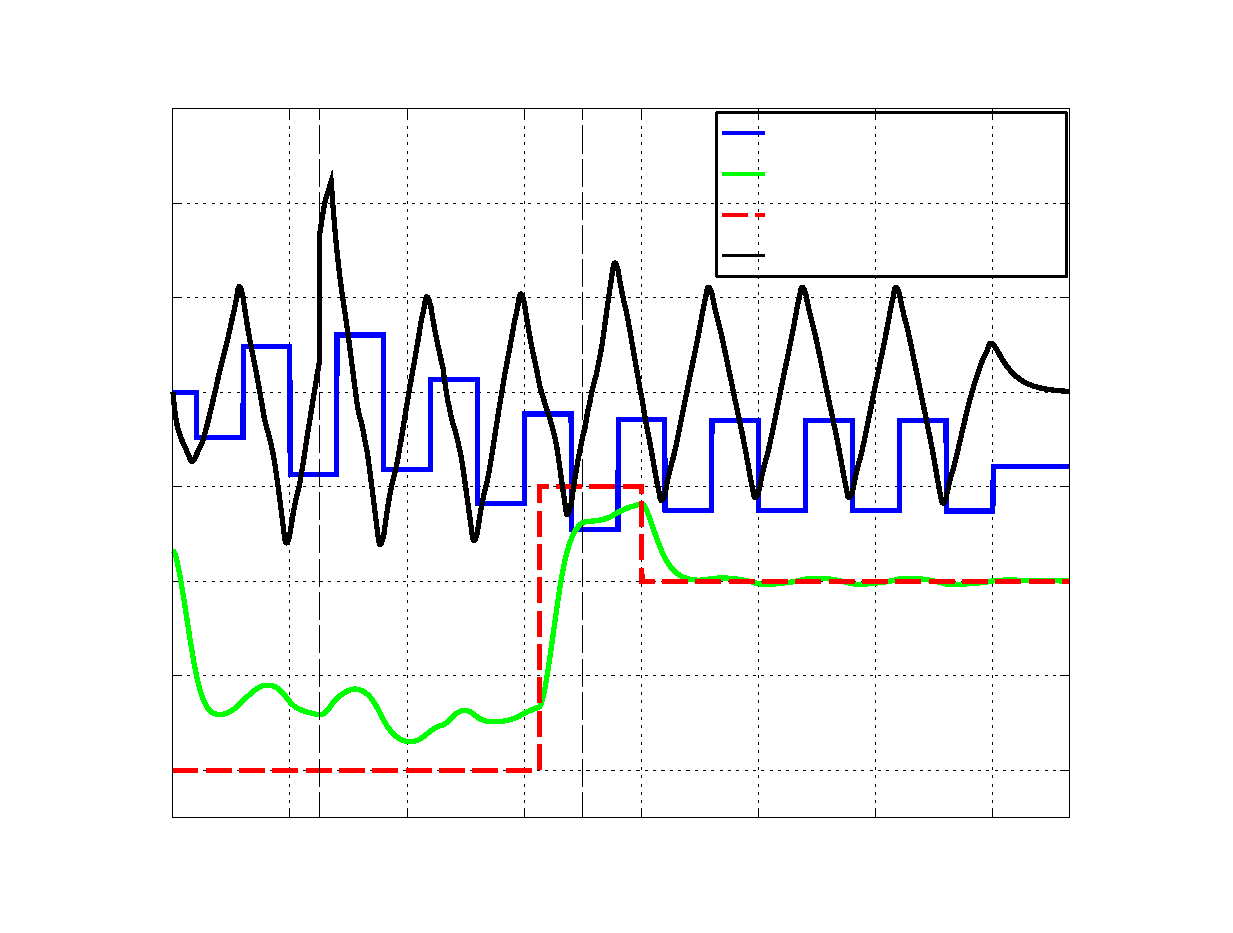
\includegraphics[trim=60   0  60  10,clip,scale=0.7]{test_16_02_XY_Y_3061-inc}
\end{picture}%
\begin{picture}(456, 422)(60,0)
\fontsize{11}{0}
\selectfont\put(74.88,42.5188){\makebox(0,0)[t]{\textcolor[rgb]{0,0,0}{{0}}}}
\fontsize{11}{0}
\selectfont\put(131.123,42.5188){\makebox(0,0)[t]{\textcolor[rgb]{0,0,0}{{2}}}}
\fontsize{11}{0}
\selectfont\put(145.184,42.5188){\makebox(0,0)[t]{\textcolor[rgb]{0,0,0}{{$\impulseC_d^y$}}}}
\fontsize{11}{0}
\selectfont\put(187.366,42.5188){\makebox(0,0)[t]{\textcolor[rgb]{0,0,0}{{4}}}}
\fontsize{11}{0}
\selectfont\put(243.609,42.5188){\makebox(0,0)[t]{\textcolor[rgb]{0,0,0}{{6}}}}
\fontsize{11}{0}
\selectfont\put(271.731,42.5188){\makebox(0,0)[t]{\textcolor[rgb]{0,0,0}{{$\impulseC_d^x$}}}}
\fontsize{11}{0}
\selectfont\put(299.852,42.5188){\makebox(0,0)[t]{\textcolor[rgb]{0,0,0}{{8}}}}
\fontsize{11}{0}
\selectfont\put(356.095,42.5188){\makebox(0,0)[t]{\textcolor[rgb]{0,0,0}{{10}}}}
\fontsize{11}{0}
\selectfont\put(412.338,42.5188){\makebox(0,0)[t]{\textcolor[rgb]{0,0,0}{{12}}}}
\fontsize{11}{0}
\selectfont\put(468.581,42.5188){\makebox(0,0)[t]{\textcolor[rgb]{0,0,0}{{14}}}}
\fontsize{11}{0}
\selectfont\put(69.8753,70.192){\makebox(0,0)[r]{\textcolor[rgb]{0,0,0}{{-0.8}}}}
\fontsize{11}{0}
\selectfont\put(69.8753,115.536){\makebox(0,0)[r]{\textcolor[rgb]{0,0,0}{{-0.6}}}}
\fontsize{11}{0}
\selectfont\put(69.8753,160.88){\makebox(0,0)[r]{\textcolor[rgb]{0,0,0}{{-0.4}}}}
\fontsize{11}{0}
\selectfont\put(69.8753,206.224){\makebox(0,0)[r]{\textcolor[rgb]{0,0,0}{{-0.2}}}}
\fontsize{11}{0}
\selectfont\put(69.8753,251.568){\makebox(0,0)[r]{\textcolor[rgb]{0,0,0}{{0}}}}
\fontsize{11}{0}
\selectfont\put(69.8753,296.912){\makebox(0,0)[r]{\textcolor[rgb]{0,0,0}{{0.2}}}}
\fontsize{11}{0}
\selectfont\put(69.8753,342.256){\makebox(0,0)[r]{\textcolor[rgb]{0,0,0}{{0.4}}}}
\fontsize{11}{0}
\selectfont\put(290.08,31.5188){\makebox(0,0)[t]{\textcolor[rgb]{0,0,0}{{simulation time $[s]$}}}}
\fontsize{11}{0}
\selectfont\put(47.8754,217.56){\rotatebox{90}{\makebox(0,0)[b]{\textcolor[rgb]{0,0,0}{{value along the $y$ axis}}}}}
\fontsize{11}{0}
\selectfont\put(136.747,310.515){\rotatebox{90}{\makebox(0,0)[l]{\textcolor[rgb]{0,0,0}{{disturbance}}}}}
\fontsize{11}{0}
\selectfont\put(263.294,310.515){\rotatebox{90}{\makebox(0,0)[l]{\textcolor[rgb]{0,0,0}{{disturbance}}}}}
\fontsize{11}{0}
\selectfont\put(361.461,375.996){\makebox(0,0)[l]{\textcolor[rgb]{0,0,0}{{Current foot position}}}}
\fontsize{11}{0}
\selectfont\put(361.461,356.326){\makebox(0,0)[l]{\textcolor[rgb]{0,0,0}{{Right hand position}}}}
\fontsize{11}{0}
\selectfont\put(361.461,336.657){\makebox(0,0)[l]{\textcolor[rgb]{0,0,0}{{Target position}}}}
\fontsize{11}{0}
\selectfont\put(361.461,316.987){\makebox(0,0)[l]{\textcolor[rgb]{0,0,0}{{CoM velocity}}}}
\end{picture}
